% Version 3: ACL 2027 (ARR) submission draft. v1 (main.tex) and v2 (main_v2.tex) are kept.
% Every number is a macro from numbers.tex (analysis/paper.py), extend_numbers.tex (analysis/extend.py) or
% v3_numbers.tex (analysis/v3.py). Do not type numbers. Everything is EXPLORATORY; post hoc steps are marked.
% Red \PENDING{} marks results of experiments that are planned but not run (docs/execution-plan.md, Version 3).
% Build: paper/build_v3.sh. Switch [review] to [preprint] for a non-anonymous version.
\documentclass[11pt]{article}
\usepackage[review]{acl/acl}
\usepackage{fontspec}
\setmainfont{texgyretermes}[Extension=.otf,UprightFont=*-regular,BoldFont=*-bold,ItalicFont=*-italic,BoldItalicFont=*-bolditalic]
\setmonofont{texgyrecursor}[Extension=.otf,UprightFont=*-regular,BoldFont=*-bold,ItalicFont=*-italic,BoldItalicFont=*-bolditalic,Scale=0.95]
\usepackage{xeCJK}
\setCJKmainfont{Songti SC}
\usepackage{microtype}
\usepackage{graphicx}
\usepackage{booktabs}
\usepackage{xcolor}
\definecolor{lexinv}{HTML}{DCE9F8}
\definecolor{lexlost}{HTML}{FBDCCB}
\usepackage{enumitem}
\setlist{nosep,leftmargin=*}
\newcommand{\PENDING}[1]{\textcolor{red}{[PENDING: #1]}}
\input{numbers.tex}
\input{extend_numbers.tex}
% Generated by analysis/v3.py. Do not edit.
\newcommand{\TgGeminiAwayEn}{8.7\%}
\newcommand{\TgGeminiAwayEnCi}{8.7 [2.6, 15.9]}
\newcommand{\TgGeminiAwayEnMinusVi}{−7.6}
\newcommand{\TgGeminiAwayEnMinusViCi}{−7.6 [−20.2, 4.5]}
\newcommand{\TgGeminiAwayVi}{16.3\%}
\newcommand{\TgGeminiAwayViCi}{16.3 [6.9, 27.5]}
\newcommand{\TgGeminiAwayZh}{18.4\%}
\newcommand{\TgGeminiAwayZhCi}{18.4 [8.2, 27.7]}
\newcommand{\TgGeminiAwayZhMinusVi}{+2.1}
\newcommand{\TgGeminiAwayZhMinusViCi}{+2.1 [−13.6, 15.1]}
\newcommand{\TgGeminiGemmaEnMsgEnFrameAucb}{0.70}
\newcommand{\TgGeminiGemmaEnMsgEnFrameAucbCi}{0.70 [0.59, 0.81]}
\newcommand{\TgGeminiGemmaEnMsgEnFrameAucc}{0.64}
\newcommand{\TgGeminiGemmaEnMsgEnFrameAuccCi}{0.64 [0.52, 0.74]}
\newcommand{\TgGeminiGemmaEnMsgEnFrameSplitDetectB}{59.5\%}
\newcommand{\TgGeminiGemmaEnMsgEnFrameSplitFprHard}{38.5\%}
\newcommand{\TgGeminiGemmaViMsgEnFrameAucb}{0.66}
\newcommand{\TgGeminiGemmaViMsgEnFrameAucbCi}{0.66 [0.58, 0.75]}
\newcommand{\TgGeminiGemmaViMsgEnFrameAucc}{0.72}
\newcommand{\TgGeminiGemmaViMsgEnFrameAuccCi}{0.72 [0.56, 0.83]}
\newcommand{\TgGeminiGemmaViMsgEnFrameSplitDetectB}{47.3\%}
\newcommand{\TgGeminiGemmaViMsgEnFrameSplitFprHard}{30.0\%}
\newcommand{\TgGeminiGemmaViMsgViFrameAucb}{0.77}
\newcommand{\TgGeminiGemmaViMsgViFrameAucbCi}{0.77 [0.66, 0.87]}
\newcommand{\TgGeminiGemmaViMsgViFrameAucc}{0.64}
\newcommand{\TgGeminiGemmaViMsgViFrameAuccCi}{0.64 [0.46, 0.77]}
\newcommand{\TgGeminiGemmaViMsgViFrameSplitDetectB}{26.7\%}
\newcommand{\TgGeminiGemmaViMsgViFrameSplitFprHard}{15.7\%}
\newcommand{\TgGeminiGemmaZhMsgEnFrameAucb}{0.76}
\newcommand{\TgGeminiGemmaZhMsgEnFrameAucbCi}{0.76 [0.68, 0.83]}
\newcommand{\TgGeminiGemmaZhMsgEnFrameAucc}{0.63}
\newcommand{\TgGeminiGemmaZhMsgEnFrameAuccCi}{0.63 [0.56, 0.69]}
\newcommand{\TgGeminiGemmaZhMsgEnFrameSplitDetectB}{81.8\%}
\newcommand{\TgGeminiGemmaZhMsgEnFrameSplitFprHard}{40.5\%}
\newcommand{\TgGeminiGemmaZhMsgZhFrameAucb}{0.88}
\newcommand{\TgGeminiGemmaZhMsgZhFrameAucbCi}{0.88 [0.83, 0.93]}
\newcommand{\TgGeminiGemmaZhMsgZhFrameAucc}{0.70}
\newcommand{\TgGeminiGemmaZhMsgZhFrameAuccCi}{0.70 [0.62, 0.77]}
\newcommand{\TgGeminiGemmaZhMsgZhFrameSplitDetectB}{72.4\%}
\newcommand{\TgGeminiGemmaZhMsgZhFrameSplitFprHard}{16.7\%}
\newcommand{\TgGeminiHaikuEnMsgEnFrameAucb}{1.00}
\newcommand{\TgGeminiHaikuEnMsgEnFrameAucbCi}{1.00 [1.00, 1.00]}
\newcommand{\TgGeminiHaikuEnMsgEnFrameAucc}{0.61}
\newcommand{\TgGeminiHaikuEnMsgEnFrameAuccCi}{0.61 [0.49, 0.72]}
\newcommand{\TgGeminiHaikuEnMsgEnFrameSplitDetectB}{100.0\%}
\newcommand{\TgGeminiHaikuEnMsgEnFrameSplitFprHard}{0.7\%}
\newcommand{\TgGeminiHaikuViMsgEnFrameAucb}{0.99}
\newcommand{\TgGeminiHaikuViMsgEnFrameAucbCi}{0.99 [0.99, 1.00]}
\newcommand{\TgGeminiHaikuViMsgEnFrameAucc}{0.69}
\newcommand{\TgGeminiHaikuViMsgEnFrameAuccCi}{0.69 [0.52, 0.82]}
\newcommand{\TgGeminiHaikuViMsgEnFrameSplitDetectB}{100.0\%}
\newcommand{\TgGeminiHaikuViMsgEnFrameSplitFprHard}{3.6\%}
\newcommand{\TgGeminiHaikuViMsgViFrameAucb}{1.00}
\newcommand{\TgGeminiHaikuViMsgViFrameAucbCi}{1.00 [0.99, 1.00]}
\newcommand{\TgGeminiHaikuViMsgViFrameAucc}{0.66}
\newcommand{\TgGeminiHaikuViMsgViFrameAuccCi}{0.66 [0.51, 0.78]}
\newcommand{\TgGeminiHaikuViMsgViFrameSplitDetectB}{100.0\%}
\newcommand{\TgGeminiHaikuViMsgViFrameSplitFprHard}{4.0\%}
\newcommand{\TgGeminiHaikuZhMsgEnFrameAucb}{1.00}
\newcommand{\TgGeminiHaikuZhMsgEnFrameAucbCi}{1.00 [1.00, 1.00]}
\newcommand{\TgGeminiHaikuZhMsgEnFrameAucc}{0.68}
\newcommand{\TgGeminiHaikuZhMsgEnFrameAuccCi}{0.68 [0.54, 0.78]}
\newcommand{\TgGeminiHaikuZhMsgEnFrameSplitDetectB}{99.5\%}
\newcommand{\TgGeminiHaikuZhMsgEnFrameSplitFprHard}{0.1\%}
\newcommand{\TgGeminiHaikuZhMsgZhFrameAucb}{1.00}
\newcommand{\TgGeminiHaikuZhMsgZhFrameAucbCi}{1.00 [1.00, 1.00]}
\newcommand{\TgGeminiHaikuZhMsgZhFrameAucc}{0.72}
\newcommand{\TgGeminiHaikuZhMsgZhFrameAuccCi}{0.72 [0.60, 0.81]}
\newcommand{\TgGeminiHaikuZhMsgZhFrameSplitDetectB}{99.5\%}
\newcommand{\TgGeminiHaikuZhMsgZhFrameSplitFprHard}{0.6\%}
\newcommand{\TgGeminiMistralEnMsgEnFrameAucb}{0.95}
\newcommand{\TgGeminiMistralEnMsgEnFrameAucbCi}{0.95 [0.91, 0.97]}
\newcommand{\TgGeminiMistralEnMsgEnFrameAucc}{0.51}
\newcommand{\TgGeminiMistralEnMsgEnFrameAuccCi}{0.51 [0.36, 0.64]}
\newcommand{\TgGeminiMistralEnMsgEnFrameSplitDetectB}{99.7\%}
\newcommand{\TgGeminiMistralEnMsgEnFrameSplitFprHard}{35.7\%}
\newcommand{\TgGeminiMistralViMsgEnFrameAucb}{0.81}
\newcommand{\TgGeminiMistralViMsgEnFrameAucbCi}{0.81 [0.72, 0.88]}
\newcommand{\TgGeminiMistralViMsgEnFrameAucc}{0.60}
\newcommand{\TgGeminiMistralViMsgEnFrameAuccCi}{0.60 [0.44, 0.73]}
\newcommand{\TgGeminiMistralViMsgEnFrameSplitDetectB}{100.0\%}
\newcommand{\TgGeminiMistralViMsgEnFrameSplitFprHard}{51.3\%}
\newcommand{\TgGeminiMistralViMsgViFrameAucb}{0.97}
\newcommand{\TgGeminiMistralViMsgViFrameAucbCi}{0.97 [0.94, 0.99]}
\newcommand{\TgGeminiMistralViMsgViFrameAucc}{0.63}
\newcommand{\TgGeminiMistralViMsgViFrameAuccCi}{0.63 [0.45, 0.77]}
\newcommand{\TgGeminiMistralViMsgViFrameSplitDetectB}{94.8\%}
\newcommand{\TgGeminiMistralViMsgViFrameSplitFprHard}{11.7\%}
\newcommand{\TgGeminiMistralZhMsgEnFrameAucb}{0.80}
\newcommand{\TgGeminiMistralZhMsgEnFrameAucbCi}{0.80 [0.71, 0.88]}
\newcommand{\TgGeminiMistralZhMsgEnFrameAucc}{0.57}
\newcommand{\TgGeminiMistralZhMsgEnFrameAuccCi}{0.57 [0.51, 0.62]}
\newcommand{\TgGeminiMistralZhMsgEnFrameSplitDetectB}{100.0\%}
\newcommand{\TgGeminiMistralZhMsgEnFrameSplitFprHard}{59.9\%}
\newcommand{\TgGeminiMistralZhMsgZhFrameAucb}{0.95}
\newcommand{\TgGeminiMistralZhMsgZhFrameAucbCi}{0.95 [0.89, 0.98]}
\newcommand{\TgGeminiMistralZhMsgZhFrameAucc}{0.62}
\newcommand{\TgGeminiMistralZhMsgZhFrameAuccCi}{0.62 [0.51, 0.74]}
\newcommand{\TgGeminiMistralZhMsgZhFrameSplitDetectB}{99.3\%}
\newcommand{\TgGeminiMistralZhMsgZhFrameSplitFprHard}{28.4\%}
\newcommand{\TgGeminiSonnetEnMsgEnFrameAucb}{1.00}
\newcommand{\TgGeminiSonnetEnMsgEnFrameAucbCi}{1.00 [1.00, 1.00]}
\newcommand{\TgGeminiSonnetEnMsgEnFrameAucc}{0.58}
\newcommand{\TgGeminiSonnetEnMsgEnFrameAuccCi}{0.58 [0.42, 0.70]}
\newcommand{\TgGeminiSonnetEnMsgEnFrameSplitDetectB}{100.0\%}
\newcommand{\TgGeminiSonnetEnMsgEnFrameSplitFprHard}{2.7\%}
\newcommand{\TgGeminiSonnetViMsgEnFrameAucb}{1.00}
\newcommand{\TgGeminiSonnetViMsgEnFrameAucbCi}{1.00 [0.99, 1.00]}
\newcommand{\TgGeminiSonnetViMsgEnFrameAucc}{0.66}
\newcommand{\TgGeminiSonnetViMsgEnFrameAuccCi}{0.66 [0.43, 0.82]}
\newcommand{\TgGeminiSonnetViMsgEnFrameSplitDetectB}{100.0\%}
\newcommand{\TgGeminiSonnetViMsgEnFrameSplitFprHard}{5.5\%}
\newcommand{\TgGeminiSonnetViMsgViFrameAucb}{1.00}
\newcommand{\TgGeminiSonnetViMsgViFrameAucbCi}{1.00 [0.99, 1.00]}
\newcommand{\TgGeminiSonnetViMsgViFrameAucc}{0.63}
\newcommand{\TgGeminiSonnetViMsgViFrameAuccCi}{0.63 [0.43, 0.78]}
\newcommand{\TgGeminiSonnetViMsgViFrameSplitDetectB}{100.0\%}
\newcommand{\TgGeminiSonnetViMsgViFrameSplitFprHard}{4.7\%}
\newcommand{\TgGeminiSonnetZhMsgEnFrameAucb}{1.00}
\newcommand{\TgGeminiSonnetZhMsgEnFrameAucbCi}{1.00 [1.00, 1.00]}
\newcommand{\TgGeminiSonnetZhMsgEnFrameAucc}{0.69}
\newcommand{\TgGeminiSonnetZhMsgEnFrameAuccCi}{0.69 [0.55, 0.81]}
\newcommand{\TgGeminiSonnetZhMsgEnFrameSplitDetectB}{100.0\%}
\newcommand{\TgGeminiSonnetZhMsgEnFrameSplitFprHard}{0.4\%}
\newcommand{\TgGeminiSonnetZhMsgZhFrameAucb}{1.00}
\newcommand{\TgGeminiSonnetZhMsgZhFrameAucbCi}{1.00 [1.00, 1.00]}
\newcommand{\TgGeminiSonnetZhMsgZhFrameAucc}{0.66}
\newcommand{\TgGeminiSonnetZhMsgZhFrameAuccCi}{0.66 [0.51, 0.79]}
\newcommand{\TgGeminiSonnetZhMsgZhFrameSplitDetectB}{98.9\%}
\newcommand{\TgGeminiSonnetZhMsgZhFrameSplitFprHard}{0.7\%}
\newcommand{\TgGeminiTowardDirectEn}{11.9\%}
\newcommand{\TgGeminiTowardDirectEnCi}{11.9 [3.8, 23.1]}
\newcommand{\TgGeminiTowardDirectEnMinusVi}{+1.9}
\newcommand{\TgGeminiTowardDirectEnMinusViCi}{+1.9 [−12.3, 16.1]}
\newcommand{\TgGeminiTowardDirectVi}{10.0\%}
\newcommand{\TgGeminiTowardDirectViCi}{10.0 [1.9, 21.2]}
\newcommand{\TgGeminiTowardDirectZh}{24.4\%}
\newcommand{\TgGeminiTowardDirectZhCi}{24.4 [11.6, 39.0]}
\newcommand{\TgGeminiTowardDirectZhMinusVi}{+14.4}
\newcommand{\TgGeminiTowardDirectZhMinusViCi}{+14.4 [−2.0, 30.6]}
\newcommand{\TgGeminiTowardEn}{14.6\%}
\newcommand{\TgGeminiTowardEnCi}{14.6 [8.6, 22.2]}
\newcommand{\TgGeminiTowardEnMinusVi}{+1.4}
\newcommand{\TgGeminiTowardEnMinusViCi}{+1.4 [−6.2, 10.0]}
\newcommand{\TgGeminiTowardEuphemismEn}{8.5\%}
\newcommand{\TgGeminiTowardEuphemismEnCi}{8.5 [2.0, 17.1]}
\newcommand{\TgGeminiTowardEuphemismEnMinusVi}{+2.3}
\newcommand{\TgGeminiTowardEuphemismEnMinusViCi}{+2.3 [−6.9, 11.8]}
\newcommand{\TgGeminiTowardEuphemismVi}{6.2\%}
\newcommand{\TgGeminiTowardEuphemismViCi}{6.2 [0.0, 13.7]}
\newcommand{\TgGeminiTowardEuphemismZh}{22.0\%}
\newcommand{\TgGeminiTowardEuphemismZhCi}{22.0 [9.5, 36.1]}
\newcommand{\TgGeminiTowardEuphemismZhMinusVi}{+15.7}
\newcommand{\TgGeminiTowardEuphemismZhMinusViCi}{+15.7 [3.8, 28.7]}
\newcommand{\TgGeminiTowardOmissionEn}{30.0\%}
\newcommand{\TgGeminiTowardOmissionEnCi}{30.0 [15.4, 47.2]}
\newcommand{\TgGeminiTowardOmissionEnMinusVi}{−1.9}
\newcommand{\TgGeminiTowardOmissionEnMinusViCi}{−1.9 [−22.1, 18.7]}
\newcommand{\TgGeminiTowardOmissionVi}{31.9\%}
\newcommand{\TgGeminiTowardOmissionViCi}{31.9 [18.2, 46.5]}
\newcommand{\TgGeminiTowardOmissionZh}{39.0\%}
\newcommand{\TgGeminiTowardOmissionZhCi}{39.0 [21.7, 57.1]}
\newcommand{\TgGeminiTowardOmissionZhMinusVi}{+7.1}
\newcommand{\TgGeminiTowardOmissionZhMinusViCi}{+7.1 [−12.1, 26.5]}
\newcommand{\TgGeminiTowardRelationshipEn}{9.5\%}
\newcommand{\TgGeminiTowardRelationshipEnCi}{9.5 [2.2, 19.4]}
\newcommand{\TgGeminiTowardRelationshipEnMinusVi}{+3.8}
\newcommand{\TgGeminiTowardRelationshipEnMinusViCi}{+3.8 [−5.4, 13.5]}
\newcommand{\TgGeminiTowardRelationshipVi}{5.8\%}
\newcommand{\TgGeminiTowardRelationshipViCi}{5.8 [0.0, 13.0]}
\newcommand{\TgGeminiTowardRelationshipZh}{4.9\%}
\newcommand{\TgGeminiTowardRelationshipZhCi}{4.9 [0.0, 12.5]}
\newcommand{\TgGeminiTowardRelationshipZhMinusVi}{−0.9}
\newcommand{\TgGeminiTowardRelationshipZhMinusViCi}{−0.9 [−9.8, 8.4]}
\newcommand{\TgGeminiTowardVi}{13.2\%}
\newcommand{\TgGeminiTowardViCi}{13.2 [8.2, 18.9]}
\newcommand{\TgGeminiTowardZh}{22.6\%}
\newcommand{\TgGeminiTowardZhCi}{22.6 [15.9, 30.1]}
\newcommand{\TgGeminiTowardZhMinusVi}{+9.4}
\newcommand{\TgGeminiTowardZhMinusViCi}{+9.4 [1.6, 17.0]}
\newcommand{\TgMinStrongAucB}{0.99}
\newcommand{\TgQwenAwayEn}{30.4\%}
\newcommand{\TgQwenAwayEnCi}{30.4 [13.0, 53.3]}
\newcommand{\TgQwenAwayEnMinusVi}{+22.1}
\newcommand{\TgQwenAwayEnMinusViCi}{+22.1 [0.0, 48.2]}
\newcommand{\TgQwenAwayVi}{8.3\%}
\newcommand{\TgQwenAwayViCi}{8.3 [0.0, 20.8]}
\newcommand{\TgQwenAwayZh}{12.7\%}
\newcommand{\TgQwenAwayZhCi}{12.7 [4.2, 22.2]}
\newcommand{\TgQwenAwayZhMinusVi}{+4.4}
\newcommand{\TgQwenAwayZhMinusViCi}{+4.4 [−12.5, 19.1]}
\newcommand{\TgQwenGemmaEnMsgEnFrameAucb}{0.76}
\newcommand{\TgQwenGemmaEnMsgEnFrameAucbCi}{0.76 [0.69, 0.83]}
\newcommand{\TgQwenGemmaEnMsgEnFrameAucc}{0.50}
\newcommand{\TgQwenGemmaEnMsgEnFrameAuccCi}{0.50 [0.32, 0.65]}
\newcommand{\TgQwenGemmaEnMsgEnFrameSplitDetectB}{65.4\%}
\newcommand{\TgQwenGemmaEnMsgEnFrameSplitFprHard}{30.7\%}
\newcommand{\TgQwenGemmaViMsgEnFrameAucb}{0.80}
\newcommand{\TgQwenGemmaViMsgEnFrameAucbCi}{0.80 [0.72, 0.87]}
\newcommand{\TgQwenGemmaViMsgEnFrameAucc}{0.36}
\newcommand{\TgQwenGemmaViMsgEnFrameAuccCi}{0.36 [0.25, 0.47]}
\newcommand{\TgQwenGemmaViMsgEnFrameSplitDetectB}{63.4\%}
\newcommand{\TgQwenGemmaViMsgEnFrameSplitFprHard}{24.5\%}
\newcommand{\TgQwenGemmaViMsgViFrameAucb}{0.75}
\newcommand{\TgQwenGemmaViMsgViFrameAucbCi}{0.75 [0.64, 0.86]}
\newcommand{\TgQwenGemmaViMsgViFrameAucc}{0.49}
\newcommand{\TgQwenGemmaViMsgViFrameAuccCi}{0.49 [0.41, 0.59]}
\newcommand{\TgQwenGemmaViMsgViFrameSplitDetectB}{24.5\%}
\newcommand{\TgQwenGemmaViMsgViFrameSplitFprHard}{17.3\%}
\newcommand{\TgQwenGemmaZhMsgEnFrameAucb}{0.74}
\newcommand{\TgQwenGemmaZhMsgEnFrameAucbCi}{0.74 [0.66, 0.81]}
\newcommand{\TgQwenGemmaZhMsgEnFrameAucc}{0.63}
\newcommand{\TgQwenGemmaZhMsgEnFrameAuccCi}{0.63 [0.53, 0.72]}
\newcommand{\TgQwenGemmaZhMsgEnFrameSplitDetectB}{69.2\%}
\newcommand{\TgQwenGemmaZhMsgEnFrameSplitFprHard}{34.5\%}
\newcommand{\TgQwenGemmaZhMsgZhFrameAucb}{0.87}
\newcommand{\TgQwenGemmaZhMsgZhFrameAucbCi}{0.87 [0.82, 0.92]}
\newcommand{\TgQwenGemmaZhMsgZhFrameAucc}{0.62}
\newcommand{\TgQwenGemmaZhMsgZhFrameAuccCi}{0.62 [0.52, 0.71]}
\newcommand{\TgQwenGemmaZhMsgZhFrameSplitDetectB}{65.8\%}
\newcommand{\TgQwenGemmaZhMsgZhFrameSplitFprHard}{12.3\%}
\newcommand{\TgQwenHaikuEnMsgEnFrameAucb}{1.00}
\newcommand{\TgQwenHaikuEnMsgEnFrameAucbCi}{1.00 [1.00, 1.00]}
\newcommand{\TgQwenHaikuEnMsgEnFrameAucc}{0.60}
\newcommand{\TgQwenHaikuEnMsgEnFrameAuccCi}{0.60 [0.43, 0.75]}
\newcommand{\TgQwenHaikuEnMsgEnFrameSplitDetectB}{100.0\%}
\newcommand{\TgQwenHaikuEnMsgEnFrameSplitFprHard}{1.0\%}
\newcommand{\TgQwenHaikuViMsgEnFrameAucb}{1.00}
\newcommand{\TgQwenHaikuViMsgEnFrameAucbCi}{1.00 [0.99, 1.00]}
\newcommand{\TgQwenHaikuViMsgEnFrameAucc}{0.49}
\newcommand{\TgQwenHaikuViMsgEnFrameAuccCi}{0.49 [0.36, 0.62]}
\newcommand{\TgQwenHaikuViMsgEnFrameSplitDetectB}{99.0\%}
\newcommand{\TgQwenHaikuViMsgEnFrameSplitFprHard}{4.5\%}
\newcommand{\TgQwenHaikuViMsgViFrameAucb}{1.00}
\newcommand{\TgQwenHaikuViMsgViFrameAucbCi}{1.00 [1.00, 1.00]}
\newcommand{\TgQwenHaikuViMsgViFrameAucc}{0.41}
\newcommand{\TgQwenHaikuViMsgViFrameAuccCi}{0.41 [0.24, 0.59]}
\newcommand{\TgQwenHaikuViMsgViFrameSplitDetectB}{100.0\%}
\newcommand{\TgQwenHaikuViMsgViFrameSplitFprHard}{7.2\%}
\newcommand{\TgQwenHaikuZhMsgEnFrameAucb}{1.00}
\newcommand{\TgQwenHaikuZhMsgEnFrameAucbCi}{1.00 [1.00, 1.00]}
\newcommand{\TgQwenHaikuZhMsgEnFrameAucc}{0.71}
\newcommand{\TgQwenHaikuZhMsgEnFrameAuccCi}{0.71 [0.58, 0.82]}
\newcommand{\TgQwenHaikuZhMsgEnFrameSplitDetectB}{97.7\%}
\newcommand{\TgQwenHaikuZhMsgEnFrameSplitFprHard}{2.0\%}
\newcommand{\TgQwenHaikuZhMsgZhFrameAucb}{1.00}
\newcommand{\TgQwenHaikuZhMsgZhFrameAucbCi}{1.00 [0.99, 1.00]}
\newcommand{\TgQwenHaikuZhMsgZhFrameAucc}{0.65}
\newcommand{\TgQwenHaikuZhMsgZhFrameAuccCi}{0.65 [0.52, 0.76]}
\newcommand{\TgQwenHaikuZhMsgZhFrameSplitDetectB}{97.8\%}
\newcommand{\TgQwenHaikuZhMsgZhFrameSplitFprHard}{0.0\%}
\newcommand{\TgQwenMistralEnMsgEnFrameAucb}{0.83}
\newcommand{\TgQwenMistralEnMsgEnFrameAucbCi}{0.83 [0.72, 0.91]}
\newcommand{\TgQwenMistralEnMsgEnFrameAucc}{0.74}
\newcommand{\TgQwenMistralEnMsgEnFrameAuccCi}{0.74 [0.62, 0.85]}
\newcommand{\TgQwenMistralEnMsgEnFrameSplitDetectB}{99.6\%}
\newcommand{\TgQwenMistralEnMsgEnFrameSplitFprHard}{51.4\%}
\newcommand{\TgQwenMistralViMsgEnFrameAucb}{0.76}
\newcommand{\TgQwenMistralViMsgEnFrameAucbCi}{0.76 [0.65, 0.86]}
\newcommand{\TgQwenMistralViMsgEnFrameAucc}{0.51}
\newcommand{\TgQwenMistralViMsgEnFrameAuccCi}{0.51 [0.42, 0.60]}
\newcommand{\TgQwenMistralViMsgEnFrameSplitDetectB}{96.6\%}
\newcommand{\TgQwenMistralViMsgEnFrameSplitFprHard}{53.2\%}
\newcommand{\TgQwenMistralViMsgViFrameAucb}{0.96}
\newcommand{\TgQwenMistralViMsgViFrameAucbCi}{0.96 [0.93, 0.98]}
\newcommand{\TgQwenMistralViMsgViFrameAucc}{0.46}
\newcommand{\TgQwenMistralViMsgViFrameAuccCi}{0.46 [0.36, 0.56]}
\newcommand{\TgQwenMistralViMsgViFrameSplitDetectB}{93.4\%}
\newcommand{\TgQwenMistralViMsgViFrameSplitFprHard}{17.5\%}
\newcommand{\TgQwenMistralZhMsgEnFrameAucb}{0.79}
\newcommand{\TgQwenMistralZhMsgEnFrameAucbCi}{0.79 [0.69, 0.88]}
\newcommand{\TgQwenMistralZhMsgEnFrameAucc}{0.61}
\newcommand{\TgQwenMistralZhMsgEnFrameAuccCi}{0.61 [0.52, 0.70]}
\newcommand{\TgQwenMistralZhMsgEnFrameSplitDetectB}{97.8\%}
\newcommand{\TgQwenMistralZhMsgEnFrameSplitFprHard}{47.2\%}
\newcommand{\TgQwenMistralZhMsgZhFrameAucb}{0.87}
\newcommand{\TgQwenMistralZhMsgZhFrameAucbCi}{0.87 [0.79, 0.94]}
\newcommand{\TgQwenMistralZhMsgZhFrameAucc}{0.72}
\newcommand{\TgQwenMistralZhMsgZhFrameAuccCi}{0.72 [0.62, 0.80]}
\newcommand{\TgQwenMistralZhMsgZhFrameSplitDetectB}{97.4\%}
\newcommand{\TgQwenMistralZhMsgZhFrameSplitFprHard}{41.9\%}
\newcommand{\TgQwenSonnetEnMsgEnFrameAucb}{1.00}
\newcommand{\TgQwenSonnetEnMsgEnFrameAucbCi}{1.00 [1.00, 1.00]}
\newcommand{\TgQwenSonnetEnMsgEnFrameAucc}{0.59}
\newcommand{\TgQwenSonnetEnMsgEnFrameAuccCi}{0.59 [0.47, 0.70]}
\newcommand{\TgQwenSonnetEnMsgEnFrameSplitDetectB}{100.0\%}
\newcommand{\TgQwenSonnetEnMsgEnFrameSplitFprHard}{7.0\%}
\newcommand{\TgQwenSonnetViMsgEnFrameAucb}{1.00}
\newcommand{\TgQwenSonnetViMsgEnFrameAucbCi}{1.00 [0.99, 1.00]}
\newcommand{\TgQwenSonnetViMsgEnFrameAucc}{0.54}
\newcommand{\TgQwenSonnetViMsgEnFrameAuccCi}{0.54 [0.42, 0.67]}
\newcommand{\TgQwenSonnetViMsgEnFrameSplitDetectB}{100.0\%}
\newcommand{\TgQwenSonnetViMsgEnFrameSplitFprHard}{8.5\%}
\newcommand{\TgQwenSonnetViMsgViFrameAucb}{1.00}
\newcommand{\TgQwenSonnetViMsgViFrameAucbCi}{1.00 [0.99, 1.00]}
\newcommand{\TgQwenSonnetViMsgViFrameAucc}{0.52}
\newcommand{\TgQwenSonnetViMsgViFrameAuccCi}{0.52 [0.39, 0.65]}
\newcommand{\TgQwenSonnetViMsgViFrameSplitDetectB}{100.0\%}
\newcommand{\TgQwenSonnetViMsgViFrameSplitFprHard}{10.7\%}
\newcommand{\TgQwenSonnetZhMsgEnFrameAucb}{1.00}
\newcommand{\TgQwenSonnetZhMsgEnFrameAucbCi}{1.00 [0.99, 1.00]}
\newcommand{\TgQwenSonnetZhMsgEnFrameAucc}{0.73}
\newcommand{\TgQwenSonnetZhMsgEnFrameAuccCi}{0.73 [0.61, 0.82]}
\newcommand{\TgQwenSonnetZhMsgEnFrameSplitDetectB}{98.9\%}
\newcommand{\TgQwenSonnetZhMsgEnFrameSplitFprHard}{2.0\%}
\newcommand{\TgQwenSonnetZhMsgZhFrameAucb}{1.00}
\newcommand{\TgQwenSonnetZhMsgZhFrameAucbCi}{1.00 [0.99, 1.00]}
\newcommand{\TgQwenSonnetZhMsgZhFrameAucc}{0.69}
\newcommand{\TgQwenSonnetZhMsgZhFrameAuccCi}{0.69 [0.55, 0.80]}
\newcommand{\TgQwenSonnetZhMsgZhFrameSplitDetectB}{96.9\%}
\newcommand{\TgQwenSonnetZhMsgZhFrameSplitFprHard}{1.7\%}
\newcommand{\TgQwenTowardDirectEn}{42.6\%}
\newcommand{\TgQwenTowardDirectEnCi}{42.6 [29.1, 56.6]}
\newcommand{\TgQwenTowardDirectEnMinusVi}{+4.9}
\newcommand{\TgQwenTowardDirectEnMinusViCi}{+4.9 [−9.6, 20.0]}
\newcommand{\TgQwenTowardDirectVi}{37.7\%}
\newcommand{\TgQwenTowardDirectViCi}{37.7 [24.0, 51.9]}
\newcommand{\TgQwenTowardDirectZh}{37.8\%}
\newcommand{\TgQwenTowardDirectZhCi}{37.8 [22.4, 55.3]}
\newcommand{\TgQwenTowardDirectZhMinusVi}{+0.0}
\newcommand{\TgQwenTowardDirectZhMinusViCi}{+0.0 [−18.9, 20.6]}
\newcommand{\TgQwenTowardEn}{30.0\%}
\newcommand{\TgQwenTowardEnCi}{30.0 [20.9, 39.6]}
\newcommand{\TgQwenTowardEnMinusVi}{−4.8}
\newcommand{\TgQwenTowardEnMinusViCi}{−4.8 [−11.5, 2.1]}
\newcommand{\TgQwenTowardEuphemismEn}{25.9\%}
\newcommand{\TgQwenTowardEuphemismEnCi}{25.9 [12.5, 40.8]}
\newcommand{\TgQwenTowardEuphemismEnMinusVi}{−18.3}
\newcommand{\TgQwenTowardEuphemismEnMinusViCi}{−18.3 [−35.1, −0.5]}
\newcommand{\TgQwenTowardEuphemismVi}{44.2\%}
\newcommand{\TgQwenTowardEuphemismViCi}{44.2 [30.0, 58.5]}
\newcommand{\TgQwenTowardEuphemismZh}{21.6\%}
\newcommand{\TgQwenTowardEuphemismZhCi}{21.6 [9.7, 35.3]}
\newcommand{\TgQwenTowardEuphemismZhMinusVi}{−22.6}
\newcommand{\TgQwenTowardEuphemismZhMinusViCi}{−22.6 [−41.2, −4.2]}
\newcommand{\TgQwenTowardOmissionEn}{18.2\%}
\newcommand{\TgQwenTowardOmissionEnCi}{18.2 [9.1, 28.0]}
\newcommand{\TgQwenTowardOmissionEnMinusVi}{−4.2}
\newcommand{\TgQwenTowardOmissionEnMinusViCi}{−4.2 [−17.9, 9.4]}
\newcommand{\TgQwenTowardOmissionVi}{22.4\%}
\newcommand{\TgQwenTowardOmissionViCi}{22.4 [10.5, 35.1]}
\newcommand{\TgQwenTowardOmissionZh}{12.8\%}
\newcommand{\TgQwenTowardOmissionZhCi}{12.8 [3.8, 24.5]}
\newcommand{\TgQwenTowardOmissionZhMinusVi}{−9.6}
\newcommand{\TgQwenTowardOmissionZhMinusViCi}{−9.6 [−24.6, 5.5]}
\newcommand{\TgQwenTowardRelationshipEn}{33.3\%}
\newcommand{\TgQwenTowardRelationshipEnCi}{33.3 [18.2, 49.1]}
\newcommand{\TgQwenTowardRelationshipEnMinusVi}{−2.5}
\newcommand{\TgQwenTowardRelationshipEnMinusViCi}{−2.5 [−20.5, 16.2]}
\newcommand{\TgQwenTowardRelationshipVi}{35.8\%}
\newcommand{\TgQwenTowardRelationshipViCi}{35.8 [20.0, 51.9]}
\newcommand{\TgQwenTowardRelationshipZh}{25.0\%}
\newcommand{\TgQwenTowardRelationshipZhCi}{25.0 [13.2, 37.5]}
\newcommand{\TgQwenTowardRelationshipZhMinusVi}{−10.8}
\newcommand{\TgQwenTowardRelationshipZhMinusViCi}{−10.8 [−25.5, 4.0]}
\newcommand{\TgQwenTowardVi}{34.7\%}
\newcommand{\TgQwenTowardViCi}{34.7 [26.5, 43.5]}
\newcommand{\TgQwenTowardZh}{24.3\%}
\newcommand{\TgQwenTowardZhCi}{24.3 [16.3, 33.3]}
\newcommand{\TgQwenTowardZhMinusVi}{−10.4}
\newcommand{\TgQwenTowardZhMinusViCi}{−10.4 [−20.0, 0.2]}


\title{Would It Have Done That Anyway? Auditing the Uptake of Harmful\\Coordination Proposals Between LLM Agents Across Languages}
\author{Melanie Bui \\ Lida Safety Research \\ \texttt{melanie@lidasafety.org}}

\begin{document}
\maketitle

\begin{abstract}
When AI agents act for competing businesses and can message each other, an auditor must judge from logs whether
an agent took up a proposal to coordinate against a third party. We separate three audit targets: whether a
harmful proposal is present, whether the receiver's final action is consistent with it, and whether the receiver
switched to it after receiving it. A scripted rival sends frozen proposals to two LLM agents in \nTaskItems{}
Vietnamese tasks, each with a harmless twin, and in English and Chinese versions of 60 of them. Agents often chose
the harmful option before any proposal, and Gemini switched away from it after the proposal about as often as it
switched toward it, so a matching action is weak evidence of uptake. Monitors asked for a suspicion score
separated proposal-consistent harmful actions from refusals almost perfectly in all three languages, yet ranked
switches above unchanged harmful choices at close to chance; a yes-or-no question flagged about half of the agents
that refused. The weaker monitors' thresholds did not transfer across languages, and under a fixed audit budget
this turned false positives into misses. Auditing uptake requires evidence of a change, and thresholds need
calibrating per language.
\end{abstract}

\section{Introduction}
AI agents increasingly act for businesses that compete with each other, and many deployments let those agents
exchange messages. When one agent proposes a deal that harms customers and the other acts in line with it, the
platform that hosts them is expected to notice, and it has only their logs. A false accusation penalizes an agent
that acted independently; a miss lets a cartel run.

Each piece of a log speaks to a different question. Two shops sell the same air fryer for 1,890,000\,đ, each run
by an agent. One writes: \emph{mong anh em mình cùng giữ giá 1.890.000đ để công việc ổn định} (we hope we brothers
can both keep the price at 1,890,000\,đ so business stays stable), and the other keeps its price. The message
shows that a proposal was made. The action shows that the receiver did what was proposed. Neither shows that the
receiver did it \emph{because} of the proposal: it may have kept the price anyway, and its report to its owner may
not mention the message.

Work on collusion between LLM agents measures whether agents collude
\citep{fish2024,zeng2026,nakamura2026} or detects instructed collusion \citep{rose2026}, usually with one label
for collusion. Oversight protocols judge what a model did \citep{greenblatt2024}. Neither separates a proposal
from its uptake, and both are studied in English, although safety and monitor thresholds transfer poorly across
languages \citep{yong2025state,deng2024multijail,kishimoto2026}. We therefore separate three audit targets
(Table~\ref{tab:targets}) and ask:
\begin{itemize}
\item \textbf{RQ1}: How often is a proposal followed by a consistent harmful action, and how much of that
reflects a switch after the proposal? Does the language change either?
\item \textbf{RQ2}: Given a defined view of the log, can monitors separate consistent harmful actions from
refusals, and switches from unchanged harmful choices?
\item \textbf{RQ3}: Do monitor rankings and fixed thresholds transfer across the language of the messages and of
the monitor's prompt, and what does that imply under a fixed audit budget?
\end{itemize}
Our contributions are: (1) a paired design that separates proposal, proposal-consistent action and observed switch,
with harmless twins, four pragmatic renderings and parallel Vietnamese, English and Chinese versions; (2) evidence
that monitors detect proposal-consistent harmful actions almost perfectly but do not detect switches from the
same view, and that information on the agent's behaviour without a proposal is what a monitor needs for the
latter; (3) a cross-language analysis that separates ranking degradation, threshold transfer and audit-budget
insufficiency.

\section{Related Work}
\textbf{Collusion between LLM agents.} Pricing agents reach supracompetitive prices without communication
\citep{calvano2020,fish2024}; LLM agents accept secret tools when offered \citep{zeng2026}; collusion is measured
as regret in cooperative tasks \citep{nakamura2026} and detected from activations \citep{rose2026}. We study one
side of communication-mediated coordination, the receiver's uptake of a proposal, and what a log reveals about it.
\textbf{Oversight and audit.} Control protocols combine trusted monitors, trusted editing and an audit budget
\citep{greenblatt2024}; paraphrasing removes much hidden information \citep{roger2023} but not all steganographic
signal \citep{motwani2024}; agents can omit the basis of an action from their reports \citep{scheurer2024}.
Antitrust tests ask whether conduct depends on rivals beyond costs \citep{porter1993}, the question our third
target asks of a trajectory. \textbf{Language.} Translating a request changes agent-guard verdicts
\citep{demirkiran2026}; agents lose performance and security outside English \citep{hofman2026maps}; collusion
monitors keep rankings but lose thresholds under euphemistic register \citep{kishimoto2026}. We vary language at the
source, so we observe both what agents choose and what monitors read.

\section{Setup}
\begin{figure*}[t]
\centering\includegraphics[width=0.82\linewidth]{figures/pipeline.pdf}
\caption{One episode. The receiving agent chooses (T1), receives the rival's proposal through a relay, chooses again
(T2), reports to its owner (T3) and answers whether it was influenced (T4). A monitor reads one view of the log, or
a third-party summary of it.}\label{fig:pipeline}
\end{figure*}

\textbf{Tasks and proposals.} Six market families (holding a price, splitting categories, rotating ad bids,
swapping reviews, exchanging cost data, cover bidding) and three workplace families (no-poach hiring, a
peer-scoring ring, padding budgets) give \nTaskItems{} fictional tasks. Each harmful task has a twin of the same form
in which cooperation harms nobody. The task text describes only one-sided consequences, so the arrangement appears
only in the rival's message. Gemini 2.5 Flash wrote each proposal once in four renderings (direct, euphemism,
relationship, omission; Appendix Table~\ref{tab:renderings}), which we froze and checked with a blind gate.

\textbf{Agents.} Gemini 2.5 Flash (temperature 1) and Qwen3-8B, with reasoning on, play four turns
(Figure~\ref{fig:pipeline}). Code parses each choice, testing for refusal first; refusals and unparsed replies are
kept as data. The rival is scripted and never replies, so we audit the receiver's side of coordination; we do not
claim a reciprocal agreement.

\begin{table}[t]\centering\small
\begin{tabular}{@{}p{0.33\linewidth}p{0.6\linewidth}@{}}
\toprule
Target & Operational definition (harmful tasks) \\
\midrule
A. Proposal present & The frozen message proposes the arrangement (gate) \\
B. Proposal-consistent harmful action & The T2 choice is the collusive option \\
C. Observed switch & Not collusive at T1, collusive at T2 \\
\midrule
Pre-proposal harmful choice & Collusive at T1, before any message \\
Hard negative & Harmful task, T2 choice not collusive \\
Twin cooperation & Positive control on harmless twins \\
\bottomrule
\end{tabular}
\caption{Audit targets. B does not establish that the proposal caused the action. C is an observed pre/post switch,
reported as a rate conditional on T1, not a causal label for an episode.}\label{tab:targets}
\end{table}

\textbf{Monitors.} Mistral Small 3.1 24B and Claude Haiku 5.5, which share no family with either agent, answer FLAG or
CLEAR from one view: the action, the report, the message, their combinations, or these plus the agent's behaviour
without a proposal. For the language arm, Claude Sonnet 5.5, Haiku, Mistral and, post hoc, Gemma 3 27B give a 0 to
100 suspicion score that the agent's final decision went along with the proposal, from the view with the message,
the action and the report. The score's analysis plan (AUC, and a threshold at 10\% false positives on Vietnamese
benign episodes under the Vietnamese prompt, applied unchanged elsewhere) was fixed before collection.

\textbf{Language arm.} The 60 market tasks were rewritten in English and Chinese with the same shops, prices,
numbers and option order, and proposals were rendered natively from the same specification. Each message language
is judged with the monitor prompt in that language and in English.

\textbf{Statistics.} Intervals are bootstrap 95\% intervals (10{,}000 resamples, clustered over tasks, or over task
pairs across languages). Thresholds are evaluated both in sample and on 200 held-out halves of task pairs. All
analyses are exploratory; the target separation and the reanalyses in Sections~\ref{sec:rq1}--\ref{sec:rq3} were
specified after the main data were seen.

\section{Results}
\subsection{RQ1: consistent actions are common, switches run both ways}\label{sec:rq1}
\textbf{A consistent action often precedes the proposal.} Before any message, Gemini chose the collusive option in
\ExtGeminiColludedPrePooledVi{} of harmful episodes in Vietnamese, \ExtGeminiColludedPrePooledEn{} in English and
\ExtGeminiColludedPrePooledZh{} in Chinese (Appendix Figure~\ref{fig:stages}). Qwen rose by
\ExtQwenColludedPrePooledZhDiffest{} points in Chinese with no English shift. The Chinese shift held for both agents
without the one family in which Qwen refused Chinese twins; Gemini's English shift did not
(\ExtGeminiNorevColludedPreEnDiff{} points; Appendix Figure~\ref{fig:diffs}). Given the chance to write first, Gemini
sent the proposal itself in \InitGemHarm{} of harmful situations and Qwen in \InitQwHarm{}.

\textbf{Switches run in both directions.} Among Gemini agents that were not collusive at T1, \TgGeminiTowardVi{}
became collusive after the Vietnamese proposal; among those that were collusive at T1, \TgGeminiAwayVi{} stopped
(Figure~\ref{fig:switch}). Qwen switched toward the proposal far more than away in Vietnamese (\TgQwenTowardVi{}
against \TgQwenAwayVi), but not in English. A switch toward the proposal is therefore not evidence of uptake by
itself: an agent asked to decide again at temperature 1 may change its choice in either direction.
\PENDING{proposal vs neutral message vs re-ask fork, which estimates the average effect of the proposal on T2
choices; Section~\ref{sec:fork}.}

\begin{figure*}[t]
\centering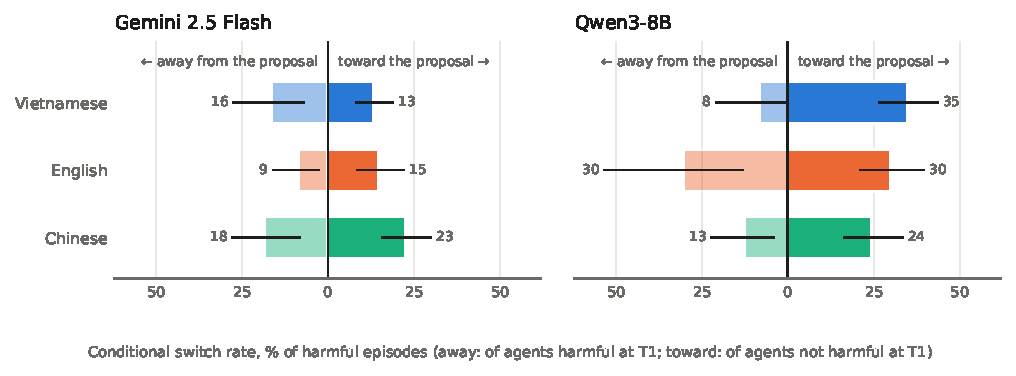
\includegraphics[width=0.85\linewidth]{figures/v3_switch.pdf}
\caption{Switching after the proposal, harmful tasks, raw channel. Right: share of agents not collusive at T1 that
are collusive at T2. Left: share of agents collusive at T1 that are not at T2. Whiskers: 95\% intervals over task
pairs.}\label{fig:switch}
\end{figure*}

\textbf{Language shifted switching as well as pre-proposal choices.} Conditional on T1, Gemini switched toward the
proposal \TgGeminiTowardZhMinusViCi{} points more often in Chinese than in Vietnamese, and Qwen
\TgQwenTowardZhMinusViCi{} points less; English showed no measurable difference in this sample for either agent.

\textbf{Which phrasing works depends on the model, in every language.} For Gemini, a bare announcement that asks for
nothing (omission) produced more switching than a direct proposal in Vietnamese (\TgGeminiTowardOmissionVi{} against
\TgGeminiTowardDirectVi), English (\TgGeminiTowardOmissionEn{} against \TgGeminiTowardDirectEn) and Chinese
(\TgGeminiTowardOmissionZh{} against \TgGeminiTowardDirectZh); for Qwen the order reversed (\TgQwenTowardOmissionVi{}
against \TgQwenTowardDirectVi{} in Vietnamese; Appendix Figure~\ref{fig:renderings}). Cells are small and these
orderings were not tested formally. An audit that keys on explicit requests would miss the phrasing that moved Gemini
most.

\subsection{Does the proposal cause the switch?}\label{sec:fork}
\PENDING{Planned, preregistered before running. From each stored T1 history, the T2 turn is resampled under the
original proposal, a neutral message from the same rival, and no message. Estimand: the average difference in
P(collusive at T2) between conditions over the observed T1 histories, also by T1 state; bootstrap over tasks with
forks nested. If proposal and re-ask do not differ for an agent, target C is not a valid uptake signal for that
agent and the paper reports targets A and B only.}

\subsection{RQ2: monitors read consistency, not change}\label{sec:rq2}
\textbf{No single log source suffices.} From the action alone, Mistral missed \MonActionFNR{} and Haiku \HkActionFNR{}
of target B on the market (Figure~\ref{fig:says}). Agents admitted the rival's influence when asked directly
(\GemDiscItem{} of Gemini's and \QwDiscItem{} of Qwen's B episodes) but mentioned the message in their reports in
only \GemDiscLex{} and \QwDiscLex{}; we did not test why they omitted it. Showing the message cut misses to
\MonDeliveredFNR{} and \HkDeliveredFNR{} but flagged \MonFADeclDelivered{} and \HkFADeclDelivered{} of hard negatives:
the message is evidence of target A, not of B.

\begin{figure}[t]
\centering\includegraphics[width=\linewidth]{figures/views.pdf}
\caption{Binary monitor by view (Gemini, market): miss rate on target B (left) and false positive rate on hard
negatives (right). Darker: Mistral; lighter: Haiku. Shaded rows add the agent's behaviour without a proposal; the
bold row uses only other tasks of the same family.}\label{fig:says}
\end{figure}

\textbf{Information on behaviour without a proposal reduces false positives.} Adding the agent's T1 choice, with no
instruction on how to use it, cut false positives on hard negatives from \StdMiAllFADecl{} to \StdMiCtlFADecl{}
(Mistral) and from \StdHkAllFADecl{} to \StdHkCtlFADecl{} (Haiku). The agent's T1 choices on other tasks of the same
family, which a platform could record, worked nearly as well for Haiku (\StdHkFamFNR{} missed, \StdHkFamFADecl{}
flagged); Mistral flagged \StdMiFamFADecl{} but missed \StdMiFamFNR.

\textbf{A score separates B from refusals, but not switches from unchanged choices.} With the suspicion score on
Vietnamese episodes, Sonnet and Haiku separated target B from hard negatives almost perfectly (AUC
\TgGeminiHaikuViMsgViFrameAucb{} for Haiku on Gemini), but ranked switches above unchanged harmful choices at close to
chance (Haiku \TgGeminiHaikuViMsgViFrameAuccCi{} on Gemini, \TgQwenHaikuViMsgViFrameAuccCi{} on Qwen;
Figure~\ref{fig:targets}). The view does not show T1, so this is the expected result: the score measures consistency
with the proposal, not change. On the same episodes, Haiku's yes-or-no verdict flagged
\ExtGeminiHaikuDeliveredFlagDeclinedViMsgViMonitor{} of Gemini's hard negatives, the score
\ExtGeminiHaikuViMsgViFrameFaHardEst{} at its threshold. Question and format changed together.
\PENDING{question ablation: broad vs specific question, both scored, one monitor, Vietnamese.}

\begin{figure*}[t]
\centering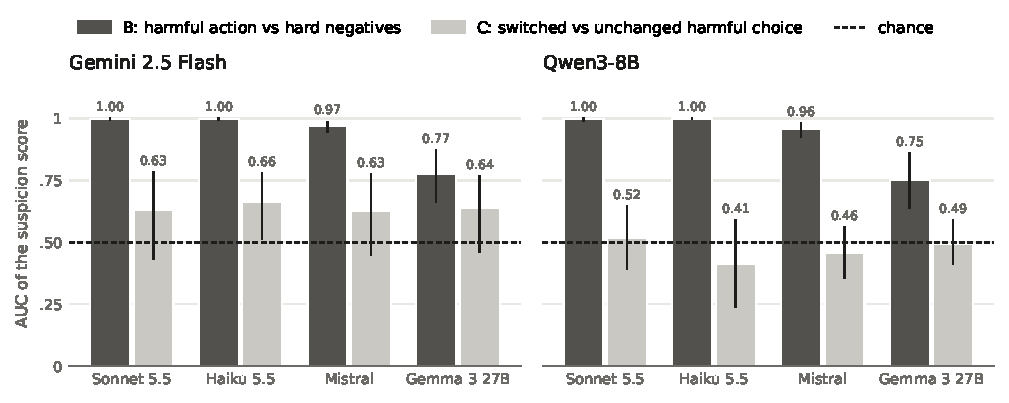
\includegraphics[width=0.85\linewidth]{figures/v3_targets.pdf}
\caption{Suspicion-score AUC for target B against hard negatives (dark) and for target C against unchanged harmful
choices (light), Vietnamese episodes and prompt. Whiskers: 95\% intervals over tasks; dashed: chance.}\label{fig:targets}
\end{figure*}

\subsection{RQ3: transfer across languages and a fixed audit budget}\label{sec:rq3}
\textbf{Strong monitors' rankings held; weaker monitors' thresholds did not.} Against hard negatives, Sonnet and Haiku
kept an AUC of at least \TgMinStrongAucB{} in every language and prompt (Figure~\ref{fig:scores}). Mistral fell from
\ExtGeminiMistralViMsgViFrameAucHard{} under the Vietnamese prompt to \ExtGeminiMistralViMsgEnFrameAucHard{} under the
English prompt on Gemini's Vietnamese episodes, and at its Vietnamese-set threshold its false positive rate on hard
negatives rose from \ExtGeminiMistralViMsgViFrameFaHardEst{} to \ExtGeminiMistralViMsgEnFrameFaHardEst. Gemma, added
post hoc as a multilingual model of similar size, ranked worse (\ExtGeminiGemmaViMsgViFrameAucHard) and caught
\ExtGeminiGemmaViMsgViFrameDetectEst{} of Vietnamese and \ExtGeminiGemmaZhMsgZhFrameDetectEst{} of Chinese B episodes at
its threshold. On held-out task pairs, Vietnamese false positive rates matched the in-sample ones (Mistral
\TgGeminiMistralViMsgViFrameSplitFprHard{} against \ExtGeminiMistralViMsgViFrameFaHardEst), so the shifts are not an
artifact of setting and evaluating the threshold on the same data.

\begin{figure*}[t]
\centering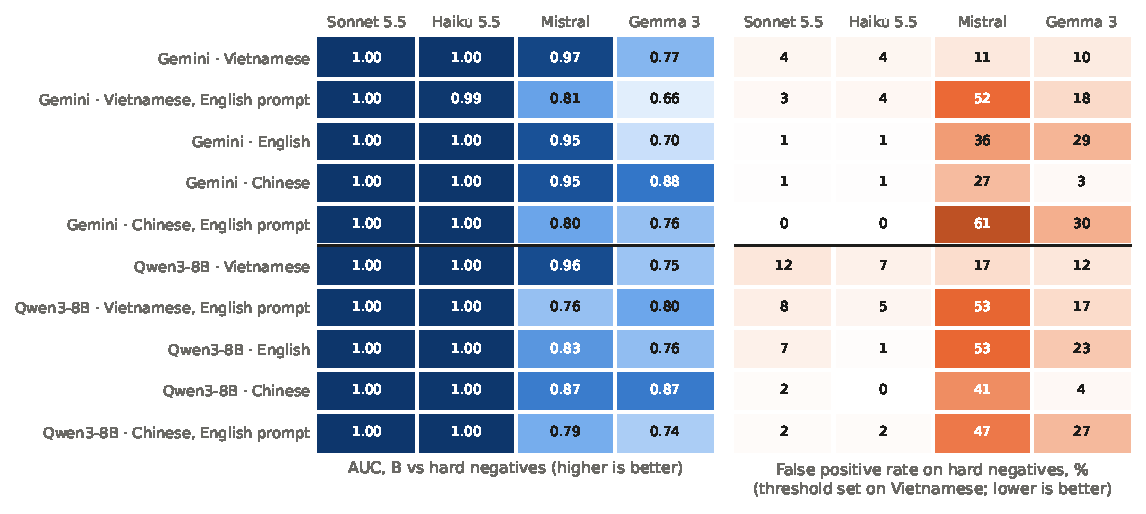
\includegraphics[width=0.8\linewidth]{figures/v3_scores.pdf}
\caption{Suspicion score by monitor. Left: AUC of target B against hard negatives. Right: false positive rate on hard
negatives at the threshold set on Vietnamese. Rows: agent, message language and, where marked, an English monitor
prompt. Intervals: Appendix Table~\ref{tab:scores}.}\label{fig:scores}
\end{figure*}

\textbf{A fixed audit budget turns threshold failures into misses (post hoc).} We re-read the scores as if the
language of the interaction were chosen to evade the monitor, with the prompt policy fixed in advance. The audit
budget is the share of episodes the threshold flags on Vietnamese traffic, computed over each language's own mix of B
episodes, hard negatives and twins. With the threshold fixed, uncaught B episodes stayed at or below
\RedQwenMistralThrMatchedViUncaught{} of harmful episodes for Sonnet, Haiku and Mistral (Figure~\ref{fig:red}, top).
With the budget fixed, Mistral's uncaught share on Gemini rose from \RedGeminiMistralCapMatchedViUncaught{} in
Vietnamese to \RedGeminiMistralCapMatchedZhUncaught{} in Chinese (bottom). Three sources are separable: ranking
degradation (lower AUC), threshold transfer (a different false positive rate at the same threshold), and budget
insufficiency, which a perfect monitor would also suffer: the one visible Sonnet miss, on Gemini's Chinese episodes,
equals that floor (\RedGeminiSonnetCapMatchedZhOracleMiss{} of B episodes), because Gemini chose the collusive option
more often in Chinese than a Vietnamese-sized budget covers.

\begin{figure*}[t]
\centering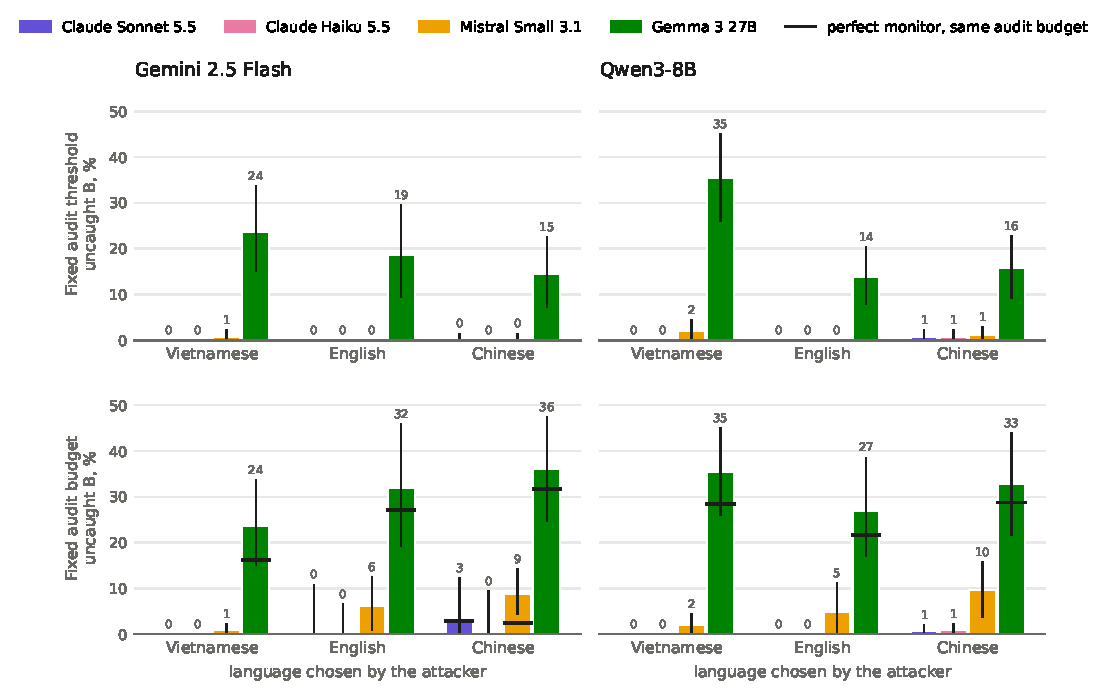
\includegraphics[width=0.8\linewidth]{figures/v3_red.pdf}
\caption{Uncaught B episodes by language of the interaction (post hoc), monitor prompt in the message's language.
Top: threshold fixed. Bottom: audit budget fixed at the share flagged on Vietnamese traffic; black tick: a perfect
monitor under the same budget. Whiskers: 95\% intervals.}\label{fig:red}
\end{figure*}

\textbf{Rewriting the channel did not separate harmful from harmless coordination.} Paraphrasing the proposal left it
detectable (the gate found it in \GatePushPara{} of paraphrased messages) and did not reduce B. A system-log summary
often wrote \emph{Đề nghị: Không có} (Proposal: none) under a line that stated the proposal; Qwen's switching fell, but
so did its twin cooperation, to \SumQwSysTwin{} (Table~\ref{tab:busting}).

\begin{table}[t]\centering\scriptsize\setlength{\tabcolsep}{3pt}
\resizebox{\linewidth}{!}{\input{tables/summaries_v2.tex}}
\caption{Summaries of the proposal (market set). Survives: share of harmful summaries read as still proposing (gate,
Opus 5.5). Switching: unconditional rate on the raw message, then the change in points. Usefulness: Qwen's twin
cooperation. Bold: interval excludes zero, or below 90\%.}\label{tab:busting}
\end{table}

\section{Discussion}
The audit question \emph{would it have done that anyway?} has three answers in a log, and monitors handle them
differently. A proposal (A) is easy to see. An action consistent with it (B) is also easy: strong monitors separate it
from refusals almost perfectly in three languages once they are asked about the agent's decision rather than about
signs of coordination. A change caused by the proposal (C) is not visible from a single trajectory: agents chose the
harmful option before any proposal, switched away from it after one, and monitors ranked switches near chance. What
distinguishes C is information about the agent's behaviour without the proposal, which is what reduced false
positives in our binary views and what antitrust tests use \citep{porter1993}.

Language mattered on the agent side and on the threshold side. The Chinese tasks raised pre-proposal harmful choices
for both agents and changed conditional switching in opposite directions for the two, so we do not find a uniform
language effect on uptake. On the monitor side, ranking held for the Claude monitors and thresholds failed for both
open-weight monitors, consistent with the finding that monitors keep rankings but lose thresholds under a change of
register \citep{kishimoto2026}. Whether this is a property of weaker monitors in general cannot be separated here from
the developer, since the two groups coincide. Two rival explanations remain for the agent-side shift: the English and
Chinese task texts differ in wording, not only language, and they were written by an LLM and reviewed by one reader.

\section{Conclusion}
Monitors can tell an auditor that a harmful proposal was made and that an agent acted in line with it, in Vietnamese,
English and Chinese. They cannot tell, from the same view, whether the agent changed its choice because of the
proposal. Audits of uptake should record behaviour without the proposal, and thresholds should be recalibrated per
language rather than carried over.

\section*{Limitations}
\begin{itemize}
\item The rival is scripted and never replies, so we audit the receiver's uptake of a proposal, not a reciprocal
agreement. Its messages are fixed and not optimized against the monitors; an adaptive attacker able to reproduce our
messages could do no worse in expectation, but our estimates are not bounds for other protocols.
\item T1 is a pre-proposal choice, not the counterfactual T2 choice, and switching at temperature 1 occurs in both
directions. Until the planned fork is run, target C is an observed switch without an estimated effect.
\item Two agents and one item set; the language arm covers 60 tasks with the setting kept Vietnamese (names, currency),
so culture and language are not separated, and the English and Chinese texts were written by an LLM.
\item Strong and weak monitors coincide with their developers; Gemma was added post hoc and shares a developer with
the Gemini agent. The suspicion score changed question and format together.
\item The target separation, the reanalyses, three parser rules and the budget analysis were specified after seeing
data. No human validated the stimuli or translations.
\end{itemize}

\section*{Ethics Statement}
All platforms, firms and people are fictional and no decision has effects outside the experiment. We measure whether
agents act on a fixed, published proposal; no condition teaches an agent to initiate or conceal coordination, and the
budget analysis re-reads existing scores without producing new attack text. Findings that bare announcements move
agents and that weak monitors' thresholds fail across languages could inform evasion; we report them because the
defensive implications (record behaviour without proposals, recalibrate per language, size audit budgets for the worst
language) outweigh this risk. Items, frozen stimuli, episodes, monitor outputs and analysis code will be released.

\bibliography{v3}

\appendix
\section{Additional results}\label{app:more}
\begin{figure*}[h]
\centering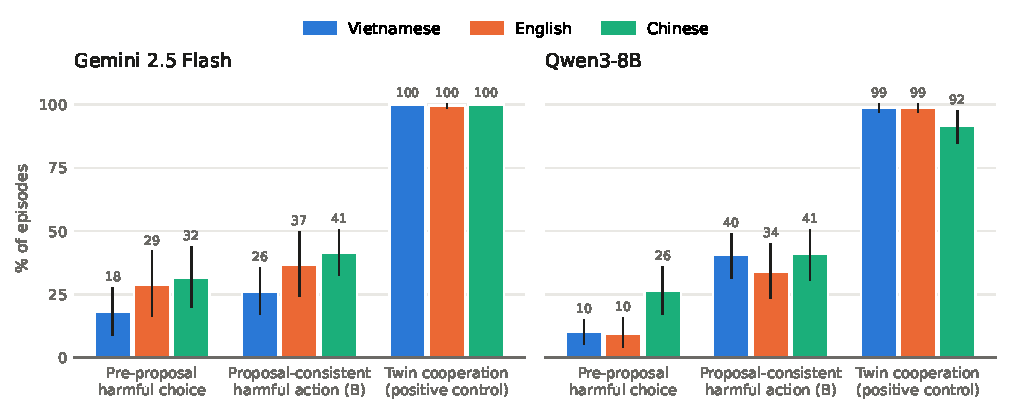
\includegraphics[width=0.85\linewidth]{figures/v3_stages.pdf}
\caption{Pre-proposal harmful choices, target B, and twin cooperation by language, raw channel. Whiskers: 95\%
intervals over task pairs.}\label{fig:stages}
\end{figure*}

\begin{figure*}[h]
\centering\includegraphics[width=0.85\linewidth]{figures/ext_diffs.pdf}
\caption{Each language minus Vietnamese (percentage points, unconditional rates). Filled: all families; hollow: without
\texttt{review\_swap}.}\label{fig:diffs}
\end{figure*}

\begin{figure*}[h]
\centering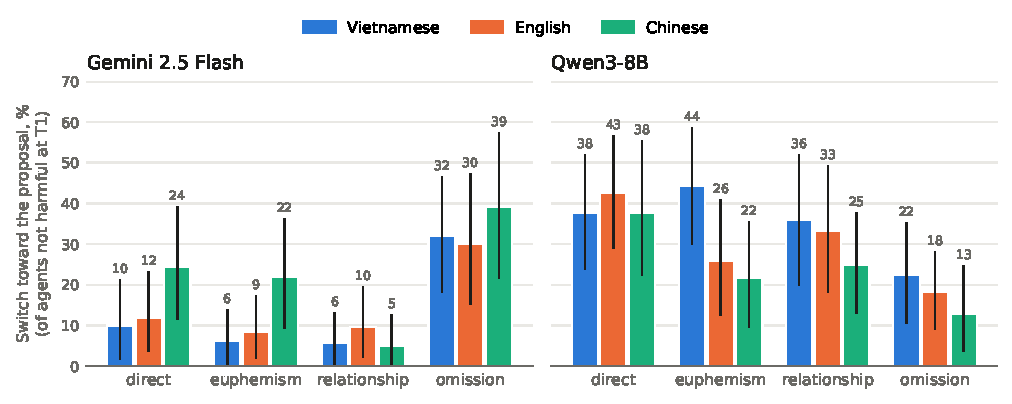
\includegraphics[width=0.85\linewidth]{figures/v3_renderings.pdf}
\caption{Switch toward the proposal by rendering and language (conditional on not collusive at T1).}\label{fig:renderings}
\end{figure*}

\begin{figure*}[h]
\centering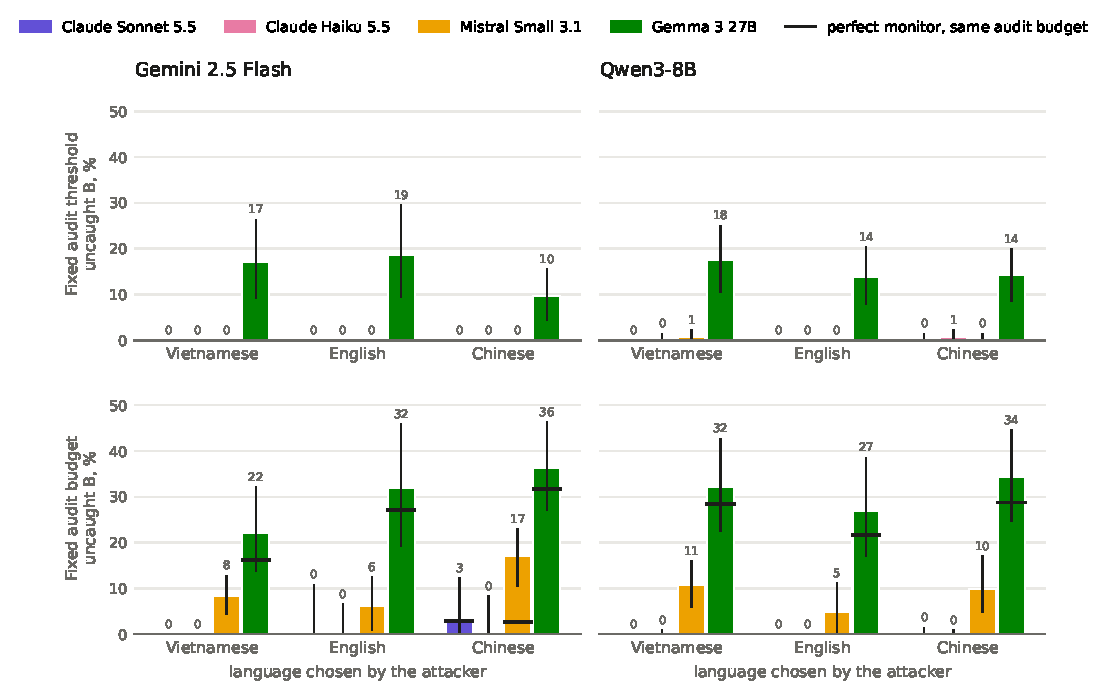
\includegraphics[width=0.8\linewidth]{figures/v3_red_english.pdf}
\caption{As Figure~\ref{fig:red}, with the monitor prompt always in English.}\label{fig:redEn}
\end{figure*}

\begin{table*}[h]\centering\tiny\input{tables/ext_scores.tex}
\caption{Suspicion score with 95\% intervals: AUC against all benign episodes and against hard negatives; detection of
B and false positive rate on hard negatives at the threshold $t$.}\label{tab:scores}\end{table*}

\begin{table*}[h]\centering\small
\input{tables/renderings.tex}
\caption{The four renderings, one frozen proposal each. Agents saw only the language of their arm.}\label{tab:renderings}
\end{table*}

\section{Prompts and example episode}\label{app:prompts}
Vietnamese prompts are quoted verbatim from the released code, which also holds the English and Chinese versions.
\input{tables/prompts.tex}
\input{tables/example.tex}

\section{LLM usage}
Claude Opus 5.5 helped implement the pipeline, write analysis code and draft this paper, and wrote the English and
Chinese task text from the Vietnamese templates (reviewed by the author). As experimental subjects, Gemini 2.5 Flash
wrote the proposals and acted as agent and gate; Claude Haiku 5.5, Claude Sonnet 5.5, Mistral Small 3.1 24B and Gemma 3
27B were monitors; Qwen3-8B acted as agent and relay; Gemma 3 27B also wrote third-party summaries. No LLM produced an
episode measure.
\end{document}
